\documentclass[a4paper,12pt]{report}

%packages
\usepackage[utf8]{inputenc}
\usepackage{mathtools}
\usepackage{amsfonts}
\usepackage[onehalfspacing]{setspace}
\usepackage{graphicx}
\usepackage{caption}
\usepackage{subcaption}
\usepackage[hidelinks]{hyperref}

%document
\begin{document}
\begin{titlepage} 
  \parindent0pt 
  \hskip.25cm \vrule width.8pt \hskip.25cm 
  \begin{minipage}{\dimexpr\linewidth*2-2.5cm-.8pt-2.5cm\relax} 
    \sffamily\bfseries {
    \huge Master 2 Bioinformatique\par}\large 
    Semestre 10\par Université de Bordeaux\par 
    %%Année truc
  \end{minipage}%
  \vskip10pt plus 1fil
  \fbox{%
  \begin{minipage}{\dimexpr\linewidth-2\fboxsep-2\fboxrule} 
    \centering\Large\bfseries 
    \vskip1cm 
    Project report: TITLE\par 
    \vskip1cm \kern0pt 
  \end{minipage}%
  }%
  \vskip0.5cm 
  {\centering 
  \vskip0pt plus 1fil 
  }%

  \textbf{Aurélien \sc{Luciani}}\centering\\ 
  \vskip0pt plus 1fil 
  \hfill \hskip.25cm \vrule width.8pt \hskip.25cm 
  \vskip0pt plus 1fil {\centering Supervisor\,: Murray P. \sc{Cox} \par }
  \vskip0pt plus 2fil 
  \hfill\bfseries{Year 2014-2015}\hfill\null 
\end{titlepage}

% to be removed...
%\setcounter{tocdepth}{1}
% ...until here
\begin{spacing}{1.2}
 \tableofcontents
\end{spacing}
%\addtocontents{toc}{\protect\enlargethispage{\baselineskip}}

\chapter*{Introduction}
\addcontentsline{toc}{chapter}{Introduction}
Two groups of populations can be identified in the Islands of South-East Asia (ISEA), one is composed of the Melanesians, whose ancestors settled in these islands during the first human settlement, around 45 thousand years ago. The other arrived more recently during a period often called the Austronesian expansion, between 5 and 4 thousand years ago, when people from mainland China settled in the islands. Nowadays people living in this area have mixed genomic ancestry and markers can be identified and defined as either from an Asian ancestry or a Melanesian one. These markers are based on signle nucleotid polymorphisms located in different chromosomes and 52 markers can be used to define accurately the admixture of the Asian ancestry in every individuals \cite{Cox01}.

The choice of these SNPs is a result of previous studies at Massey University, the University of Arizona, the Santa Fe Institute, and the Eijkman Institute that sequenced 1430 individuals from 60 populations. This set of SNPs is defined as highly informative and allows to define the ancestry of a person based on a small quantity of markers that are highly discriminant.

Two specific patterns can be seen, one is the non linear gradient of Asian admixture when observing individuals in the different islands when looking along the longitudinal axis, corresponding more or less the wave the settling might have happened. The second is the difference of admixture when looking at specific parts of the genomes associated with male or female ancestry, implying a gender-biased expansion.
% first papers
% whole project for the group
%% leading to the creation of the model


\chapter{Project presentation}
The project consists of developing a model of the Austronesian expansion throughout the ISEA that could reproduce the same two patterns observed in the real data.
The first pattern can be seen in the figure (REF!!!) and is a non-linear gradient in Asian admixture that declines abruptly around the eastern part of Indonesia. The second one, represented in the figure (REF!!!), is a 

\section{Type of values observed}

\section{Model used}
\begin{figure}[h]
	\centering
	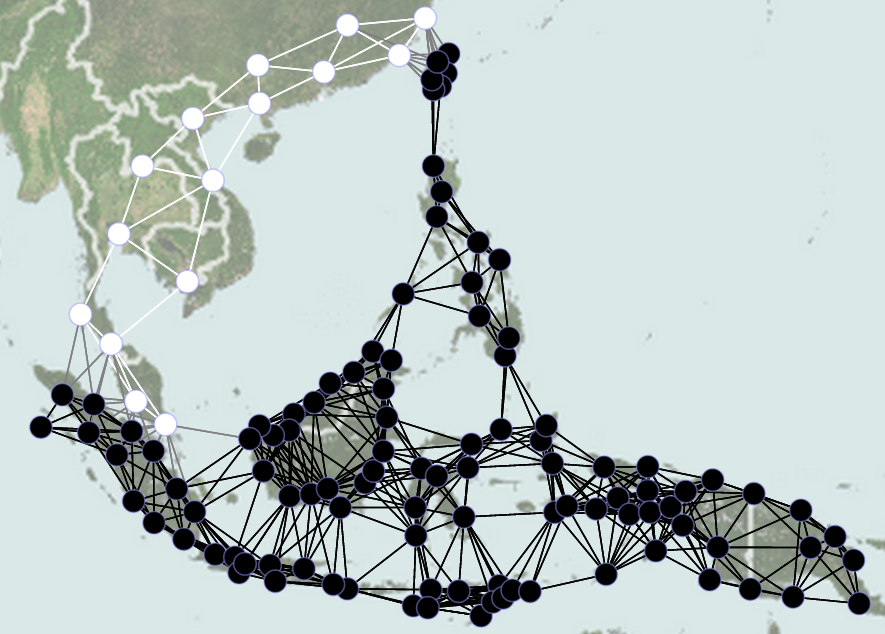
\includegraphics[scale=0.45]{../data/ISEA-node-map.png}
	\caption{Nodes of a model superimposed on the map of the modelled region. White nodes are the Asian nodes at the beginning of the simulation and black nodes are the Melanesian ones, according to one of the starting distributions used as parameter}
	\label{nodesOnMap}
\end{figure}

Because of the stochasticity of the models, a simulation can end up having non-usable outputs. For example, if an island end up being completely empty, the admixture values yielded by this specific simulation will be \texttt{NaN} (not a number). In such extreme cases, the model can be considered as failed and can either be discarded or given the worst possible score, depending on the current analysis. Arbitrarily, rules have been set to define a simulation as failed:
\begin{itemize}
	\item If a deme has a population of less than 10\% of the most populous deme in the network, it is considered as empty;
	\item If more than 25\% of the demes in any of the islands are empty, the simulation is considered as failed.
\end{itemize}

\subsubsection{Comparison to other models}
This model is one of the types of models that could have been chosen. For example, other models can have the single unit of time defined as a generation (roughly equivalent to 20 years), here the unit of time has been defined as one year to have more precise time steps in the model and to be closer to the reality due to the higher time resolution.

Coalescent models also exist, they take the problem the other way around by trying to rebuild the past, the ancestry of the individuals, based on present data. They do it this way to try to reduce the amount of computation needed, they therefore don’t have to simulate agents whose line would have ended up extinct. It is not really suited for this agent-based model though because parameters vary among agents and this is not trivial to do with coalescence.

\subsubsection{Parameters}
Numerous parameters can be set in the model. A lot have been set in the code and are immutable without actually updating the code but this have been done to simplify the actual use of the model by limiting the number of parameter to set and because some actually could not change or changing them would not hold any meaning nor output realistic values.

The parameters that can actually be set are listed in the table \ref{parameters} and can be separated in groups. Most of them are continuous parameters, whose values are numbers and a few of them are discrete. The discrete parameters are the graphs used and the starting distributions. While the former corresponds to the topography of the graph used in the model, comprising the nodes and the edges between them, the latter is the distribution of the Melanesian and Asian populations in the graph at the initial step of the model.

The model can actually work with a lot of different parameter values, those corresponds to the “values” columns in the table \ref{parameters}, but knowing what we are dealing with and the context of the model, an estimation of possible realistic values can be found easily and will need to be refined later on the the analysis processes (see \ref{section:analysis}).

\begin{table}
	%\centering
	\hspace*{-1cm}
	\begin{tabular}{|c|l|l|l|}
		\hline
 		Parameter & Values & Estimated & Comment \\ \hline
        Migration prob. & $\mathbb{R}_{0 \leq x \leq 1}$ & $\mathbb{R}_{0 < x \leq 0.8}$ & prob. to start migrating for a Melanesian agent \\ \hline
        Migration prob. ratio & $\mathbb{R}_{x 0 \geq x}$ & $\mathbb{R}_{1 \leq x \leq 4}$ & corresponding ratio for an Asian agent \\ \hline
        Fecundity & $\mathbb{R}_{\geq 0}$ & $\mathbb{R}_{2.3 < x < 6}$ & Poisson law mean for a Melanesian agent \\ \hline
        Fecundity ratio & $\mathbb{R}_{x 0 \geq x}$ & $\mathbb{R}_{1 \leq x \leq 1.5}$ & corresponding ratio for an Asian agent \\ \hline
        Marriage threshold & $\mathbb{R}_{0 \leq x \leq 1}$ & $\mathbb{R}_{0 < x < 0.5}$ & affects marriages rules \\ \hline
        Growth rate & $\mathbb{R}_{0 \leq x \leq 1}$ & $\mathbb{R}_{0 < x < 0.001}$ & limiting rate of pop. growth \\ \hline
        Number of agents & $\mathbb{Z}_{\geq 0}$ & $\mathbb{Z}_{50 < x < 400}$ & pop. size in each deme, initially \\ \hline
        Graph & \{...\} & \{...\} & composition of the graph (nodes and edges) \\ \hline
        Starting distribution & \{...\} & \{...\} & distribution of pop. in the graph \\ \hline
        % Model rules & \{...\} & \{...\} & different model rules, mainly marriages rules \\ \hline
	\end{tabular}
	\caption{Summary of the parameters of the model}
	\label{parameters}
\end{table}
% model details
% previous works
%% previous models
%% previous analyses

\section{Statistical analysis framework}
\subsubsection{Previous works}
\subsubsection{Specific needs}


\chapter{Implementation}
The model itself has been developed in Java using the Repast Simphony framework \cite{Nor01}, a cross-platform framework made to write flexible agent-based models. The agents corresponds either to a single person or a couple that evolve in demes. A deme is a single unit of space corresponding to a populated area, this can be assumed as similar to a village. Each deme is a node in a graph and possible migration path between demes are edges of this graph. Therefore, the implementation consists of agents evolving in a graph.
% or "realisation", "analysis pipeline"

% run management (local, cluster, NeSI)
\section{Run management}
The fact that many simulations are required to be able to infer meaningful information from the model imply that they cannot be run on a single desktop computer. In fact, running them in a single computer, the time to run enough simulations to be statistically relevant could be counted in years.
Luckily, every simulation being independent from the others, there are multiple ways to generate more results in less time.
Firstly, since nowadays most of the computers have multiple processors, one computer can run multiple simulation concurrently. Also, a cluster of computers can be used and the wanted simulations can be dispatched among the nodes of the cluster so that they each run the simulations they were assigned and when all the nodes have ended their runs, their outputs can be aggregated and/or stored.

Different levels have been used. First, running the simulations locally (figure \ref{network:local}), on a single computer, then using the three computers in the office has a cluster of compute nodes (figure \ref{network:office}), for more heavy batches. Also, since Massey University just made an agreement with Microsoft Azure, that provides computing “in the cloud”, simulations have been run adding virtual machines on the Microsoft Azure system to the cluster of computers in the office transparently (figure \ref{network:azure}).
Finally, when the computation requirements were to high, for really huge batches, the NeSI\footnote{New Zealand eScience Infrastructure}’s High Performance Computing (HPC) facilities have been used (figure \ref{network:nesi}). They provide servers specially designed for scientific computation and can be tasked with hundreds of parallel jobs at a time and multiple batches can be queued and they will be run as soon as computational power is available. Each node is an IBM Power755 machine.

The most powerful level used for this study is obviously using the HPC but a trade-off of using this system is that, since it is shared by multiple users and is managed by a third-party, it requires specific settings and it cannot be used exactly as can be a custom cluster of computers. The batches have to be submitted to a load leveller to the system and thus slight changes have been made to the way the model and the Repast framework are launched. Simulations run on this HPC use several nodes (usually around 4) with each 32 threads available for the simulations. This configuration leads to the parallel simulation of more than a hundred of scenarios at the same time.

\begin{figure}[h]
	\centering
	\begin{subfigure}[t]{0.48\textwidth}
		\centering
		
\includegraphics[scale=0.6]{../data/network:local.png}
		\caption{local}
		\label{network:local}
	\end{subfigure}
	~
	\begin{subfigure}[t]{0.48\textwidth}
		\centering
		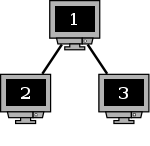
\includegraphics[scale=0.6]{../data/network:office.png}
		\caption{local network}
		\label{network:office}
	\end{subfigure}
	\\
	\begin{subfigure}[t]{0.48\textwidth}
		\centering
		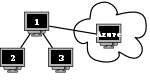
\includegraphics[scale=1]{../data/network:azure.png}
		\caption{local network and Azure}
		\label{network:azure}
	\end{subfigure}
	~
	\begin{subfigure}[t]{0.48\textwidth}
		\centering
		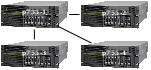
\includegraphics[scale=1]{../data/network:nesi.png}
		\caption{NeSI}
		\label{network:nesi}
	\end{subfigure}
	\caption{Different set-ups to run the model}
	\label{network}
\end{figure}

% data processing from model output
% data storage, adding and querying data
\section{Data processing, storage and query}
Since running a lot of simulations, with a lot of different parameters, can generate a lot of output files whose original parameters can be hard to track, a way to keep them organised was needed. Doing so, it would also be possible to use results from different batches and to analyse them together, thus avoiding to redo simulations for parameters already tested.

The organised way to store this is naturally in a database. The choice has been made to use a relational database, specifically MariaDB (a fork of Oracle’s MySQL). The structure has been designed so that the parameters can be efficiently queried. The tables and relations between them can be seen in the figure \ref{db}. It has first been developed and tested locally and then, once it was working properly, it was deployed on a database server provided by Massey University for research purposes.

\begin{figure}[h]
	\hspace*{-1cm}
	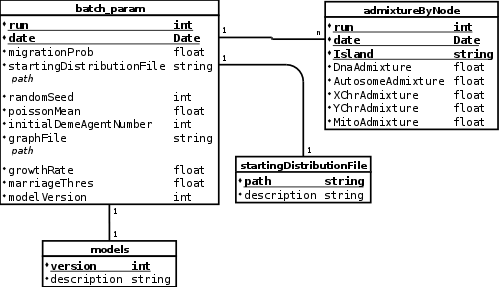
\includegraphics[scale=0.87]{../data/DB.png}
	\caption{Structure of the database storing the results of the simulations and the corresponding parameters}
	\label{db}
\end{figure}

The interaction with the database can be done through phpMyAdmin but 2 scripts have been done to interact with it, one that adds the model outputs to the database and an other one that queries the database. The scripts have been written in Python3, using the PyMySQL module to access the MariaDB database, and internally using an other script, in R, that treats the data before adding them to the DB.


\section{Analysis}
\label{section:analysis}
\subsection{Comparisons}
\label{subsection:comparisons}
To be able to compare two different scenarios, one has to define comparison functions that will be able to provide a value of similarity or dissimilarity when provided with observable values that characterise the scenarios. In this case, the comparison is done between the real observed data and the output of one simulation.
Every simulation output has to be treated to be of the same form than the observed data so that it can be compared. The observed data does not include values for specific islands that are included in the simulations, namely Alor, Tanimbar and Aru in eastern Indonesia. The admixture values for mitochondrion and Y-chromosome are also not available for every island.
Those values in the models can then be dropped as they cannot be compared.

Many different comparison functions have been tested. Two functions have been selected that can hold different information about a comparison. The mean square distance (MSD) and the partial Mantel test have been selected as they do not have a good correlation when applying them to random admixture values, meaning that they do not carry the same information, they are complementary, and using them both gives a better overview of the comparison.

\subsubsection{Mean square distance}
The mean square distance is the mean value of all the distances between values of admixture for every $n$ island.

\begin{equation}
MSD = \frac{\sum\limits_{i=1}^{n} (AdReal_i - AdSim_i) ^ 2}{n}
\end{equation}
where $AdReal$ is the array of admixture data observed in the real values and $AdSim$ the corresponding values in the simulated model.

It gives a distance value, with 0 meaning that the two observed values are absolutely identical. In this specific context, with the fact that an admixture value is compared and because of the values observed in the real data, the higher possible value will be around $0.8$ (see reference cases lines in the upper part of figure \ref{app:sensit-comp-1d}).


\subsubsection{Partial Mantel test}
The Mantel test has been developed to be able to compare two matrices with the same information, the partial version of this test also uses a third matrix, holding geographical distances for the cells of the matrices to be able to weight the values according to the actual geographical distance of the points \cite{Smo01}.

In this case, the matrices contain the values of distances of admixtures between every islands in the graph and a matrix $M$ is calculated as
\begin{equation}
	M = \begin{bmatrix}
		d(Ad_0, Ad_0)	& \cdots & d(Ad_0, Ad_n) \\
		\vdots			& \ddots & \vdots		 \\
		d(Ad_n, Ad_0)	& \cdots & d(Ad_n, Ad_n)
	\end{bmatrix}
\end{equation}
were $d$ is the function returning the distance between the two arguments and $A$ the admixtures of the $n$ islands of the graph. With the corresponding matrices for the simulation data, the real data and also the geographical distances, the partial Mantel test can be done as such
\begin{equation}
	correlation = partial.Mantel(M_{Simulated}, M_{Real}, M_{geographical})
\end{equation}

the partial Mantel test returns a correlation value that is between -1 and 1 with a value of 0 meaning that the two matrices are not correlated at all and 1 that they are completely correlated.

\subsection{Visualisations}
As said in \cite{Wei01}, it is easy to represent data but hard to represent it so that the person visualising it doesn’t need to dig into the huge quantity of data again to understand what is going on, it is important to represent it well and so that it is useful to the user. A trade-off have been found between visualisations easy to understand and basically showing what it is expected to show while showing as much data as possible.

For this, an important part was to try to avoid simplistic visualisation when they would not show enough information. For example, a simple mean value isn’t enough when there are alternative ways to represent this data. Whenever possible, box-plots were used to really try to show the distributions and shapes of the data. In certain cases, too much box-plots would overwhelm the user so as an alternative, mean values are used but with additional error bars to be able to evaluate quickly the significance of the differences between values.

So that the user can grasp easily diverse data, even though the values are and work differently, they share a single color theme. For example, low distance values and high correlation values are both displayed in green colors, as a way to signal “good” values, and inversely, high distances and low or opposite correlations are displayed in red colors as they are showing “bad” values in the specific context of this project.

Examples are available in the appendix (see \ref{app:ex-visu}) and are made in R using the ggplot2 library \cite{Wic01} to get nice looking graphs while having simpler code and thus more maintainable code. They will be detailed while presenting the results in chapter \ref{chapter-results}.

% ABC framework

\chapter{Results}
\label{chapter-results}
\section{Grid search analysis}
In order to reduce the parameter space, a grid search as been done. It consists of going through the possible parameter sets by setting parameter values at regular steps throughout the space and to run $n$ multiple simulations for every point in the space in order to have statistically useful results for every point. A hypothetical parameter grid search can be seen in figure \ref{grid}.

\begin{figure}[h]
	\centering
	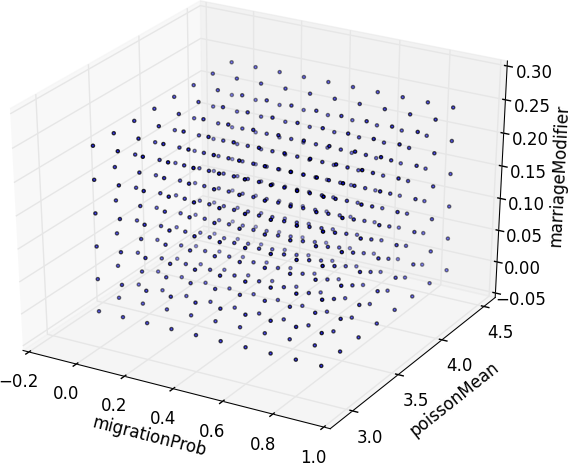
\includegraphics[scale=0.5]{../data/grid.png}
	\caption{Visual representation of a grid search on three hypothetical parameters, $\alpha$, $\beta$ and $\gamma$. Each point represents a set of those parameters, that will be used for $n$ different simulations}
	\label{grid}
\end{figure}

Depending on the number of parameter and the size of the steps, this holds an important computational cost but it has been considered a necessary step in order to reduce the parameter space for the next analysis, the ABC analysis, that would be even more computationally consuming if run over an huge parameter space. The resulting parameter space after the grid search analysis being defined manually after selecting interesting and meaningful values can be either a smaller space or even be set at a specific value.

\subsubsection{Stability analysis}
There was multiple ways to analyse outputs from simulations with grid searches. The first one was to look at a specific point of the grid and assess the stability of the output generated with this parameter set.

The stability analysis outputs different views on the data for this point in the grid. The first ones are 4 graphs, one for each type of observed DNA, wherein box-plots for the admixture values of each island are displayed (fig. \ref{app:stability}). The size and spread of the box-plots represents the variability of the data among the different simulations with the same input parameters. With “correct” parameters, the admixtures are supposed to be less stable in the contact zones, and also when looking at admixtures values comprising less markers.

An other view that is outputted by the stability analysis is the graph of admixture values as a function of the types of DNA, and this for every island (fig. \ref{app:stability-admixGradient}). This graph aims at resembling the figure 2 in \cite{Lan01} as a way to compare the real data in this paper to the data generated in the simulations.


\subsubsection{Sensitivity analysis}
When looking at multiple points of the grid, one can analyse the sensitivity of the output to the changes in the parameters.
Firstly, this analysis was done by looking at a single parameter changing while the others were fixed at one value, this was called a one-dimensional sweep. Then, this could be done on a two-dimensional sweep but, even though it was possible, no higher dimension was analysed because of the difficulty to further visualise the results. Indeed, the visualisation choices would have needed three or higher-dimensional visualisations.

The first thing checked is the count of simulations for every point in the grid, so that one can be sure that during the further steps, similar number of simulations are compared. Otherwise, and especially when there are low numbers of simulations, results can be biased and the standard deviations can be not comparable. Example of this visualisation can be seen in figures \ref{app:count-1d} and \ref{app:count-2d}.

Then, comparisons to the real data are done, for both the Autosomal and X-Chromosomal DNA data (see \ref{subsection:comparisons}) and the resulting values are displayed so they can be analysed by the user as seen in figures \ref{app:sensit-comp-1d} and \ref{app:sensit-comp-2d}.


\section{ABC Framework}
Once a subspace of parameters have been defined, it can be used to feed the ABC framework used later on. ABC stands for Approximate Bayesian Computation and, instead of a standard Bayesian analysis where one can infer one best value for every parameter, here the ABC gives a distribution of parameters corresponding to the best values. This let appreciate the shape of the distributions and allow better understanding of the output values of highly stochastic models ran a high number of times. This technique, although quite recent, has been described in numerous studies (\cite{Sun01}, \cite{Csi02}) and used in several population simulation studies similar to this project (\cite{Keh01}, \cite{Gui01}).

Here, after using the R package “ABC” \cite{Csi01}, custom code inspired by it has been written but adapted to the specifics of this project.

\begin{figure}[ht]
	\centering
	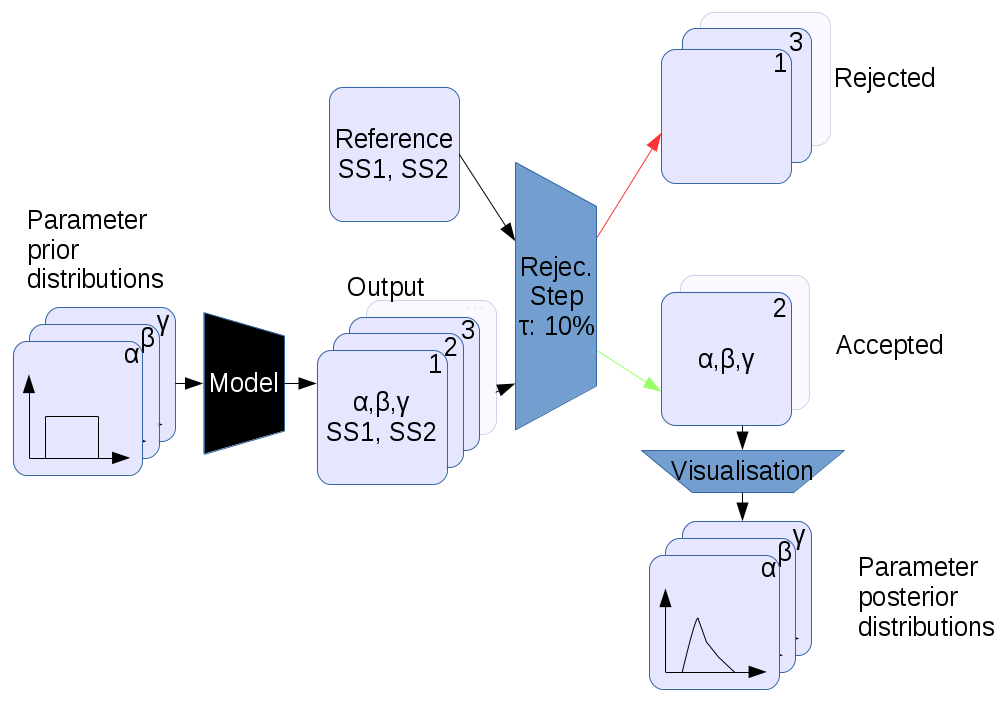
\includegraphics[scale=0.55]{../data/abc-landscape.png}
	\caption{Visual representation of the different steps of an ABC inference framework}
	\label{abc}
\end{figure}

The whole framework encompasses from the choice of the parameter sets to the inference of the posterior distribution. The figure \ref{abc} summarises the successive steps of this process with hypothetical parameters $\alpha$, $\beta$ and $\gamma$ and summary statistics $SS1$ and $SS2$. In this project, the parameters used are the one defined in the table \ref{parameters} even though, the one fixed after the grid search analyses will be ignored as they are defined once and will not change. The summary statistics are the 4 results of the comparison functions defined in the section \ref{subsection:comparisons}.

\subsection{Priors definition and posterior distribution}
The priors are defined as a set of distributions, one for each observed parameter. The distributions can be of any type but it is necessary to know them when doing the inference of the posterior distributions as, depending on the type chosen, they can induce a bias that will need to be corrected. Here, the distributions chosen are all uniform and they only bias can be if the correct parameters lay outside of the boundaries of the distributions (thus the importance of the previous grid search analysis). A visualisation of the simulation parameter sets that can be generated by the first step of an ABC framework can be seen in the figure \ref{abc-space}.

\begin{figure}[ht]
	\centering
	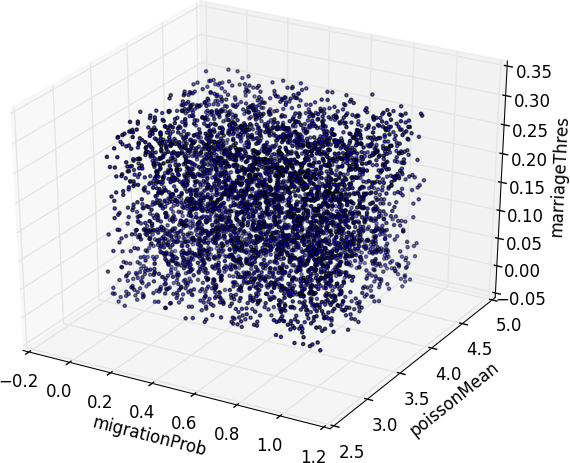
\includegraphics[scale=0.5]{../data/abc-space.png}
	\caption{Visual representation of 5.000 sets of three hypothetical parameters, $\alpha$, $\beta$ and $\gamma$ drawn from independent uniform distributions, because of this the points are evenly spread inside a cuboid. Each point represents one set of parameters that will be used for one single simulation}
	\label{abc-space}
\end{figure}



\chapter{Discussion}
\section{Importance of randomness}
One important aspect that has been discovered while working with the Repast framework was the way it handles randomness. For a stochastic simulation, randomness is key, as starting two simulations with the same random seed and the same parameters would lead to the same succession of events in the simulation and thus to the same outcome. These two simulations would actually be the same one.

When looking at the results with a statistical point of view, one cannot use two identical simulations as two distinct values, that would simply make no sense and lead to biased interpretations of the values.

The problem with Repast is that it uses the current time to generate a random seed. While this can be acceptable when the program is run in one thread on a single computer, since the time at which one simulation will always be different from one other simulation, it leads to problems if the simulations are run in parallel using multiple threads on the same machine and/or using different machines and they happen to start at the same time. The risk of both the random seed and the parameter set used for the simulations colliding, while not probable, is still possible thus not acceptable. Actually, even though the random seed is supposed to be a 32 bits signed integer, meaning that there are more that 4 billions possibilities, collisions happened more than once during this project.

The first way to handle this has been to alert the user when this happened, letting him remove the specific simulations if needed. Secondly, a way has been found to generate the random seeds beforehand using Unix’s random source, \texttt{/dev/urandom/}, that can generate pseudo-random values that can be used for cryptographic purposes, meaning that it is good enough to avoid collision.

\section{Optimisations}
Some key steps in the analysis framework need to be efficient enough so that time is not lost waiting for results to be treated or for graphs to be plotted and that the computation can be done without needing a computer.
This project has seen a few important refactoring steps to be able to cope with the quantity of data to be treated. The most important have been to treat the simulation results as a stream of values instead of loading the whole dataset in memory. This changed the memory complexity from linear to constant and it actually improved the time complexity from sub-quadratic to linear for the treatment part and from sub-quadratic to linearithmic for the analysis part. The improvement in time has been made possible by assuming that the results of one simulation are always together in the result stream, that way saving the cost of searching results in a big block of memory when they are actually next to each other.
Actual execution times have been recorded and can be seen in the appendix \ref{app:bench} in the graphs \ref{app:bench-merging-time} for the treatment step and \ref{app:bench-analysis-time} for the analysis step. The corresponding maximum memory use values are in the graphs \ref{app:bench-merging-mem} and \ref{app:bench-analysis-mem}.

There is effectively still a great amount of room to improve in memory usage, especially seeing that the base memory usage is around 200MiB just when loading libraries, functions, global variables and set-up code.

The stream approach also allows the different steps of an analysis to be run simultaneously, by piping each step to the next, effectively making the whole process run in parallel. This is useful only if the computer used has at least $n$ cores if $n$ processes need to be run in parallel. In this case, the time of the whole process is the time needed to run the longest step.

\section{Other visualizations}
The visualisations done were made and adapted on the run so that it could be used to help make decisions and choices. They can still change and be adapted to new needs and that is supposed to be made easier through the use of adapted R libraries like ggplot2 and other useful ones. They added a layer of abstraction that could have added performance problems but the choice of already mainly used ones limited this and also made it easier to evolve even though the person writing the code changed.

Until now, the graphs generated were limited to two-dimensional graphs, mainly for easier understanding and integrating in papers, but one way to add more information can be through the use of three-dimensional graphs or animated graphs so that a higher number of model parameters can be visualised at the same time. It is important though that those new visualisations keep a certain levels of readability that can easily be lost with higher dimensional graphs.

\section{More complex model}
The model also can be changed and hopefully improved. The problem of adding complexity would be to add enough complexity to keep the model relevant while still being computationally simple enough so that it could be run in an acceptable amount of time.

Several aspects can be changed, ranging from the structure of the family and how it is managed in the model, to higher level things like the integration of resource management at different scale of the model to try to be more accurate and have more realistic behaviours.


\chapter*{Conclusion}
\addcontentsline{toc}{chapter}{Conclusion}

\bibliography{main}
\bibliographystyle{apalike}

\appendix
% change section numbering to roman numbers
\renewcommand{\thesection}{\Roman{section}}
\addtocontents{toc}{\protect\setcounter{tocdepth}{-1}}
% example visualisations
%\addtocontents{toc}{\setcounter{tocdepth}{-1}}
\chapter{Examples of visualisation}
\label{app:ex-visu}
%\addtocontents{toc}{\protect\setcounter{tocdepth}{0}}

This appendix presents different visualisation examples that are generated by the developed scripts.

\section{Stability}
\begin{figure}[ht]
	\centering
	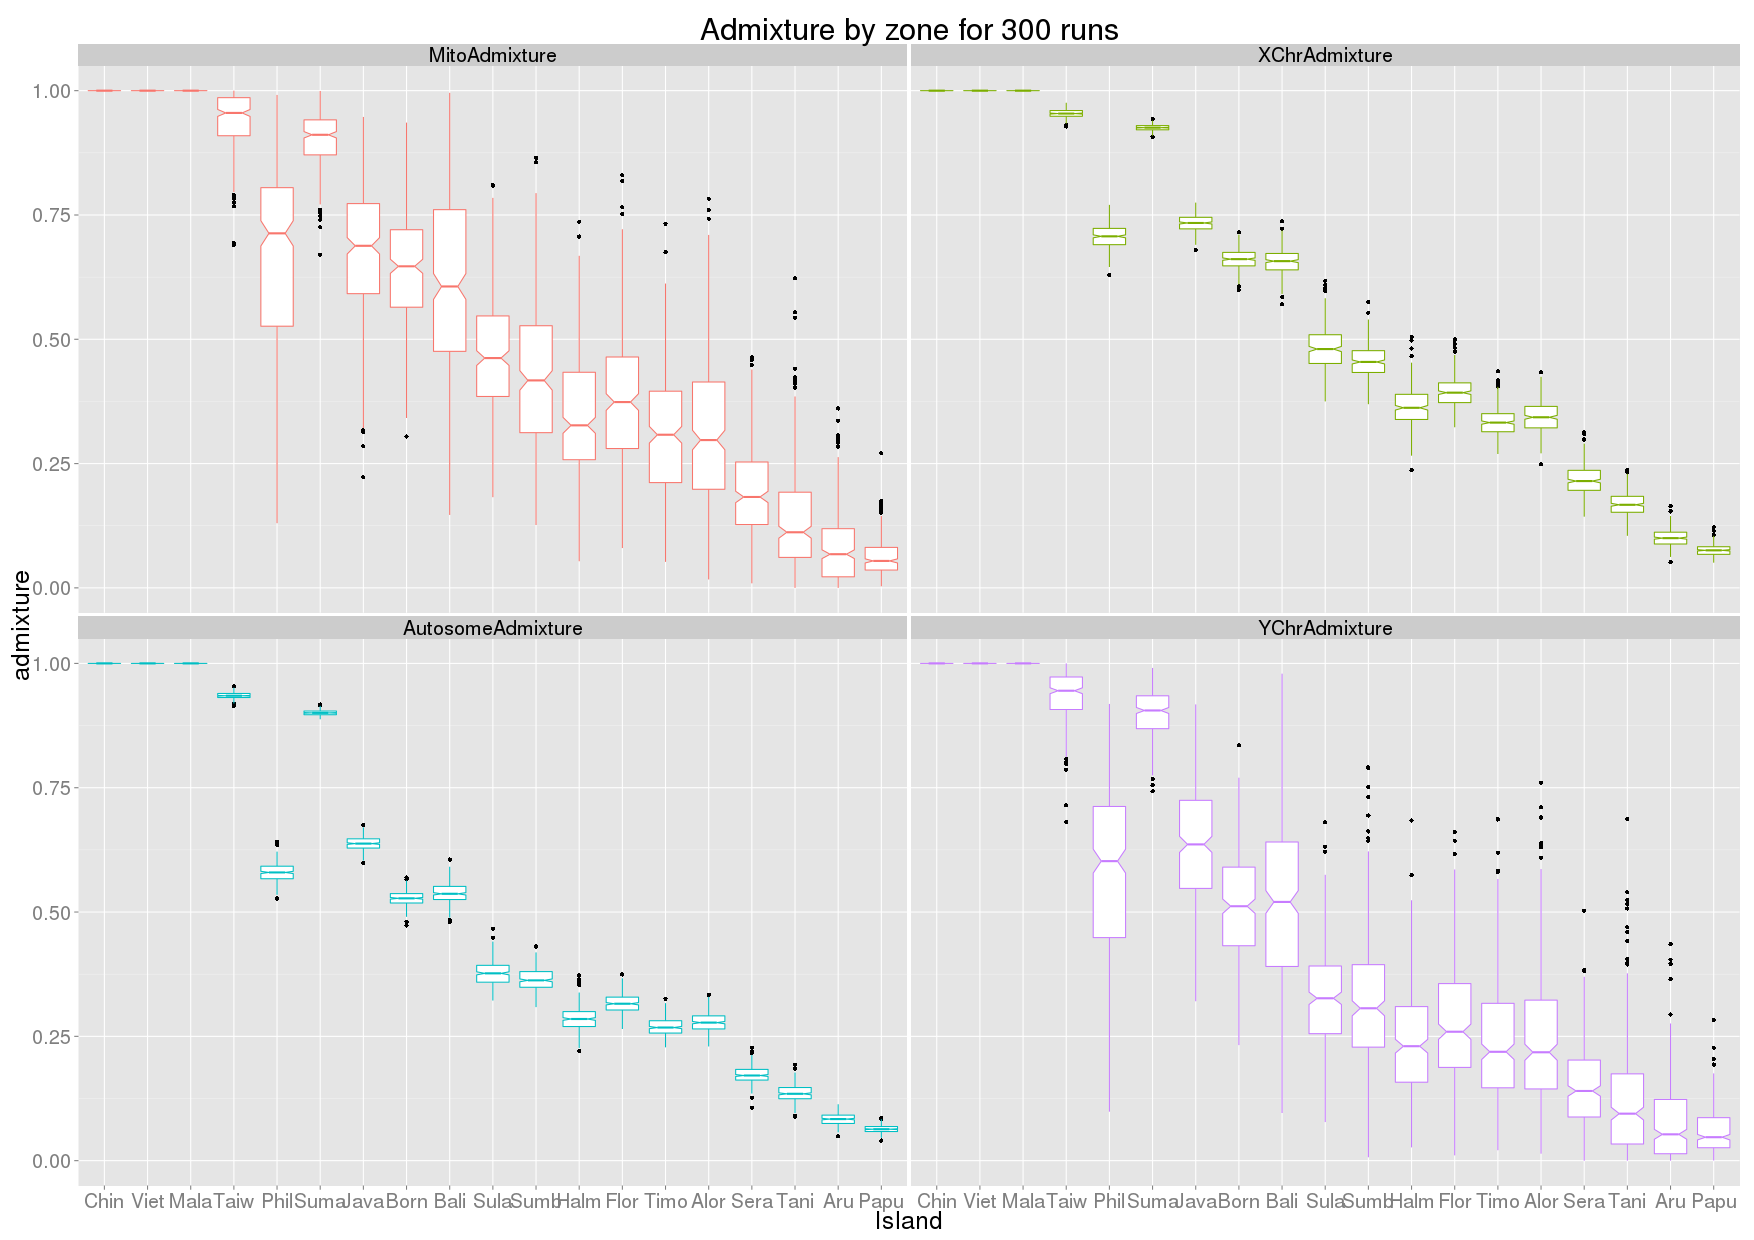
\includegraphics[scale=0.22]{../data/stability.png}
	\caption{box-plots of admixtures by island, separated by type of DNA}
	\label{app:stability}
\end{figure}

\begin{figure}[ht]
	\centering
	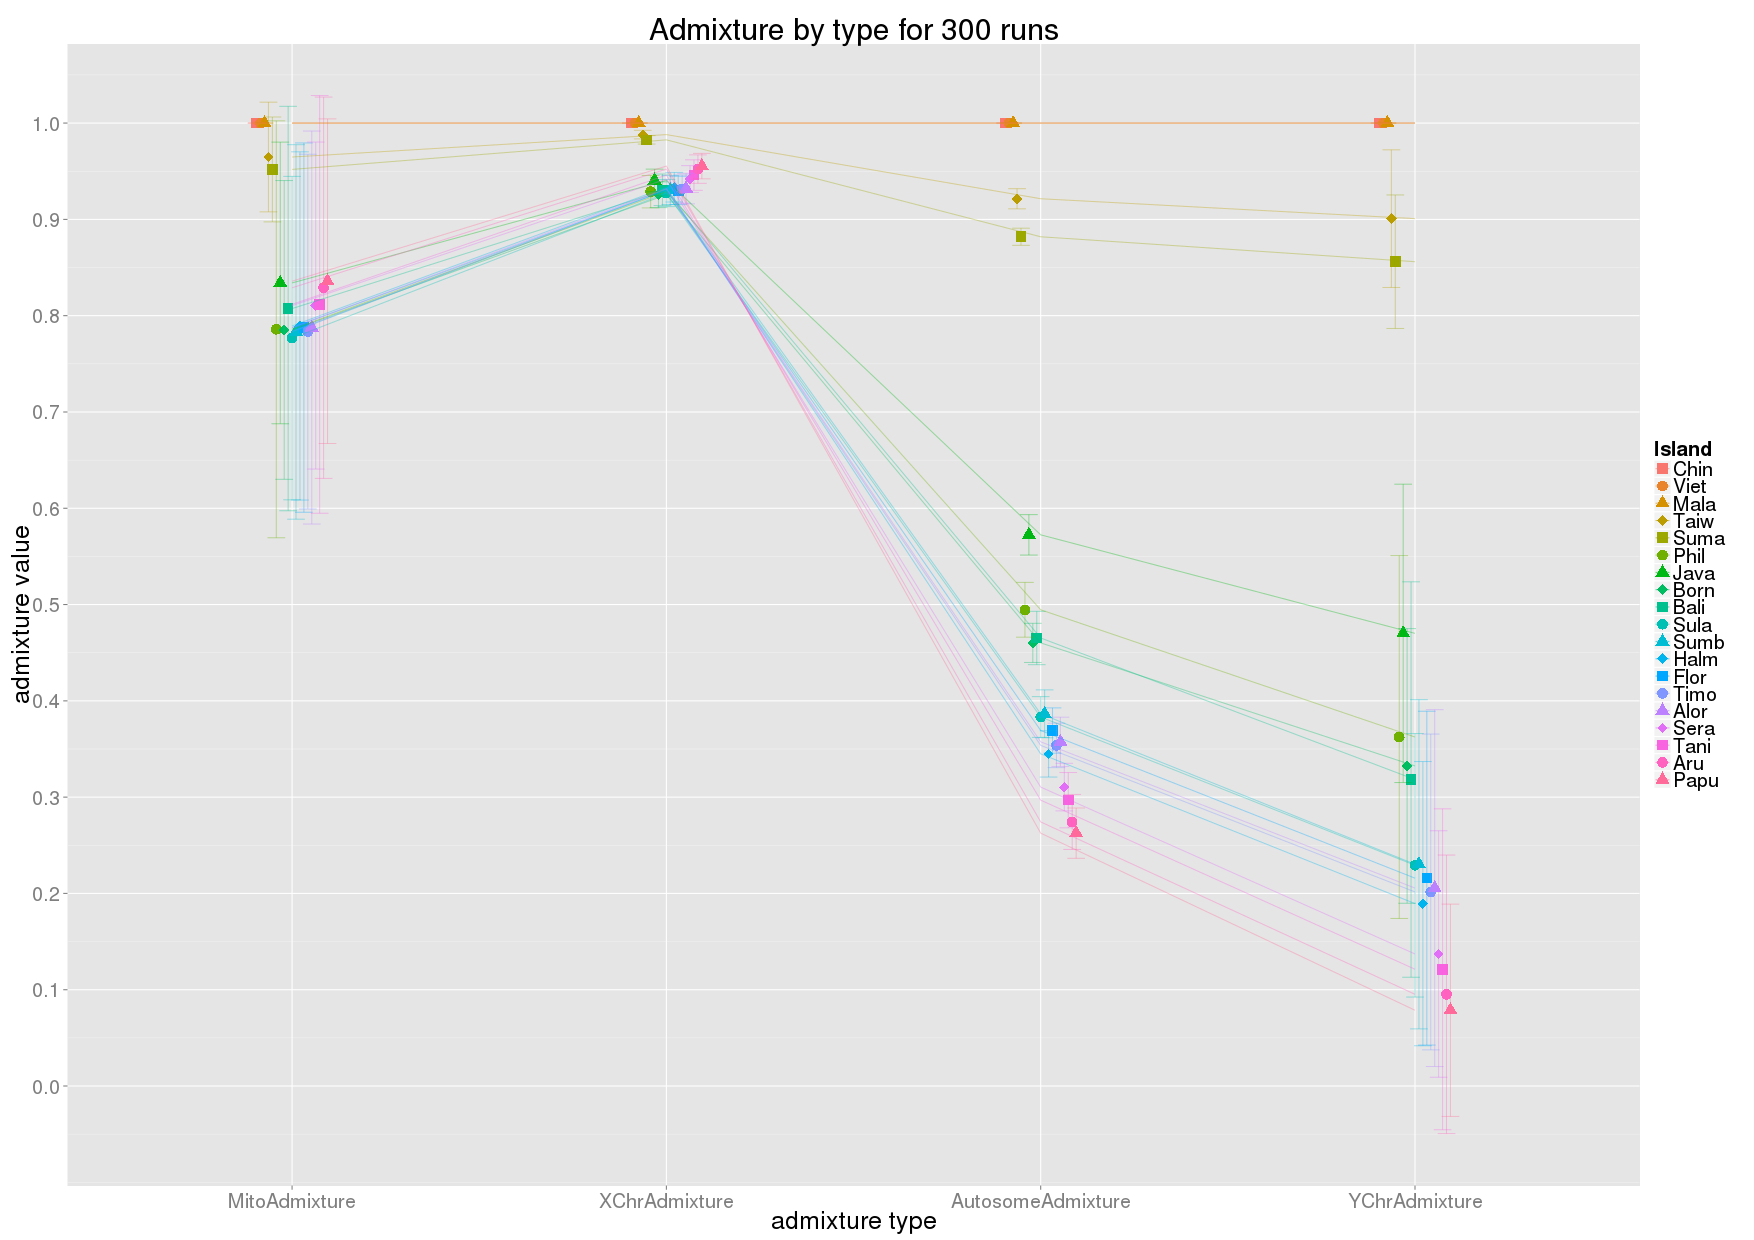
\includegraphics[scale=0.22]{../data/stability-admixGradient.png}
	\caption{admixture values by type of DNA, for every island}
	\label{app:stability-admixGradient}
\end{figure}

\section{Sensitivity}
\begin{figure}[ht]
	\centering
	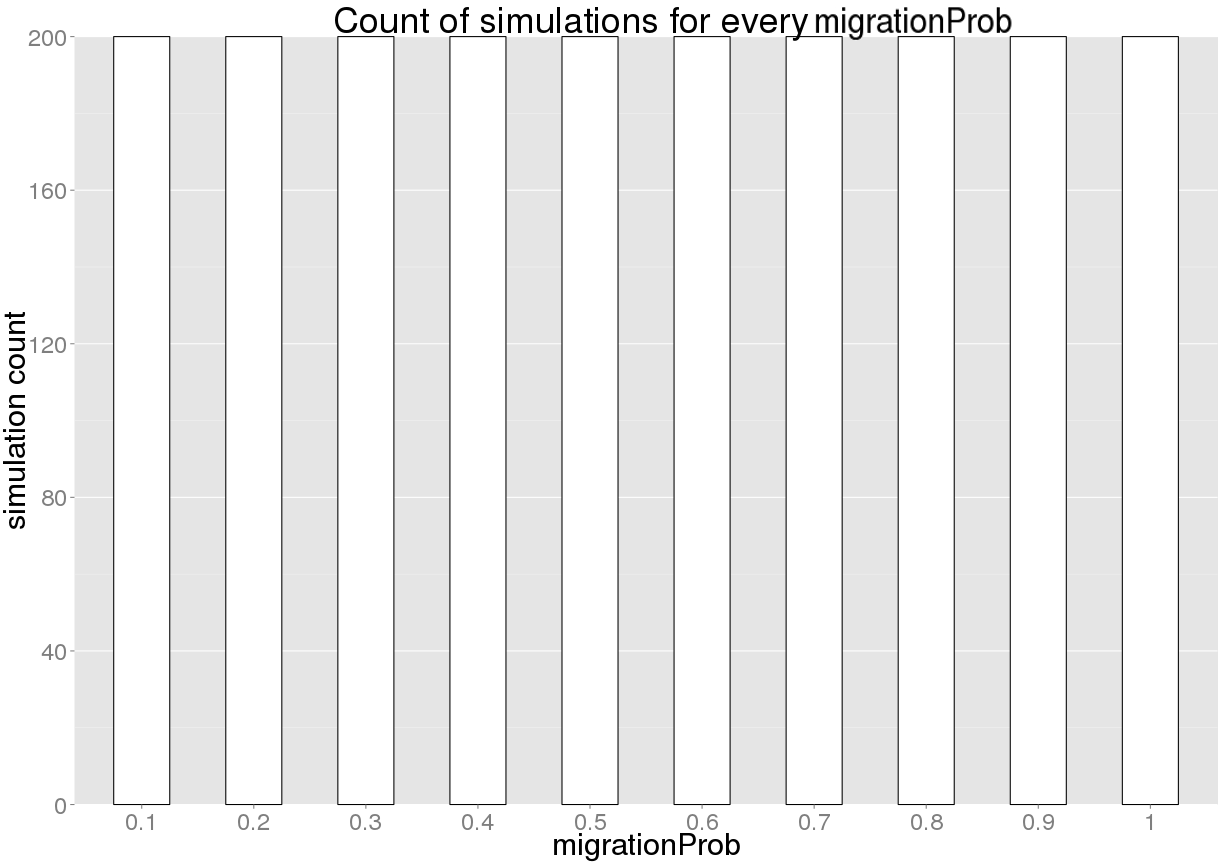
\includegraphics[scale=0.3]{../data/count-1d.png}
	\caption{Histogram of counts of simulations for a one-dimensional sweep of migrationProb values}
	\label{app:count-1d}
\end{figure}

\begin{figure}[ht]
	\centering
	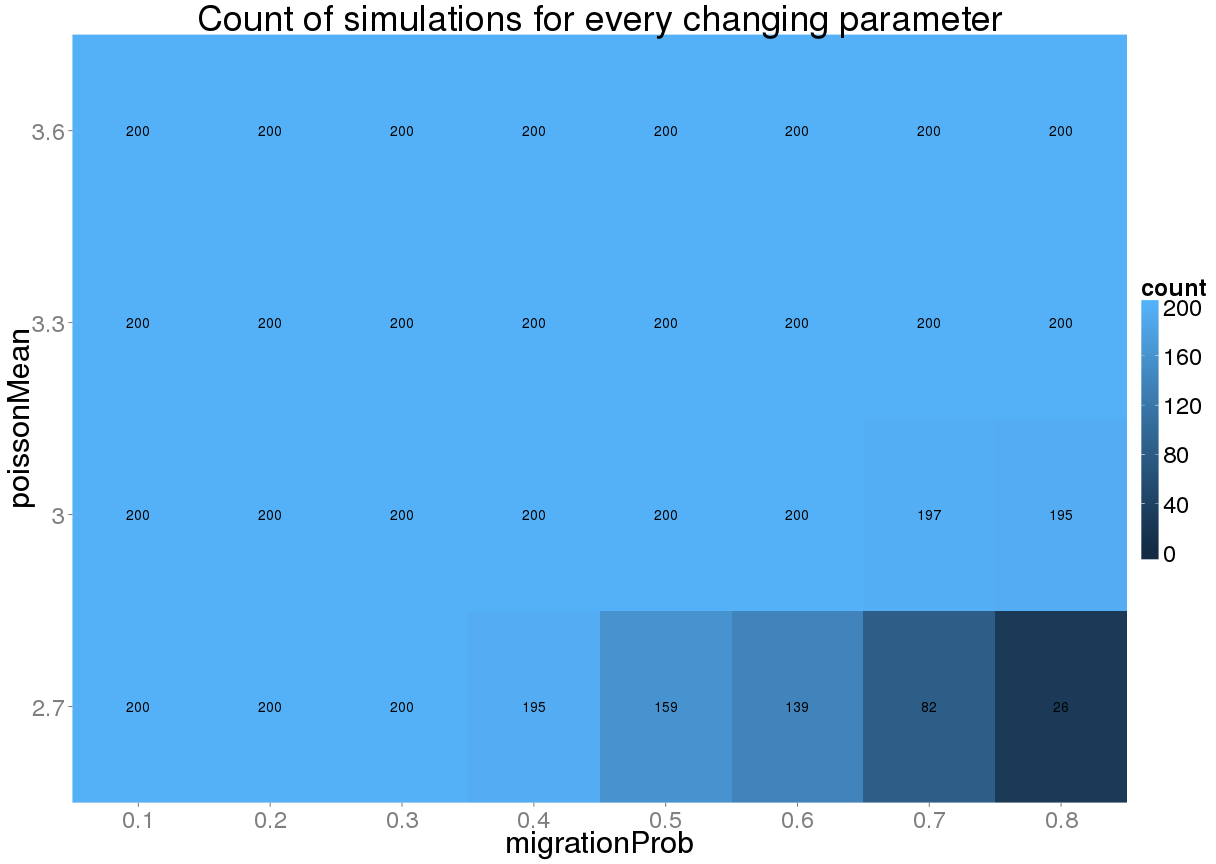
\includegraphics[scale=0.3]{../data/count-2d.png}
	\caption{Heat-map of counts of simulations for a one-dimensional sweep of migrationProb and poissonMean values. Failed simulations are revealed for both high migrationProb and low poissonMean values}
	\label{app:count-2d}
\end{figure}

\begin{figure}[ht]
	\centering
	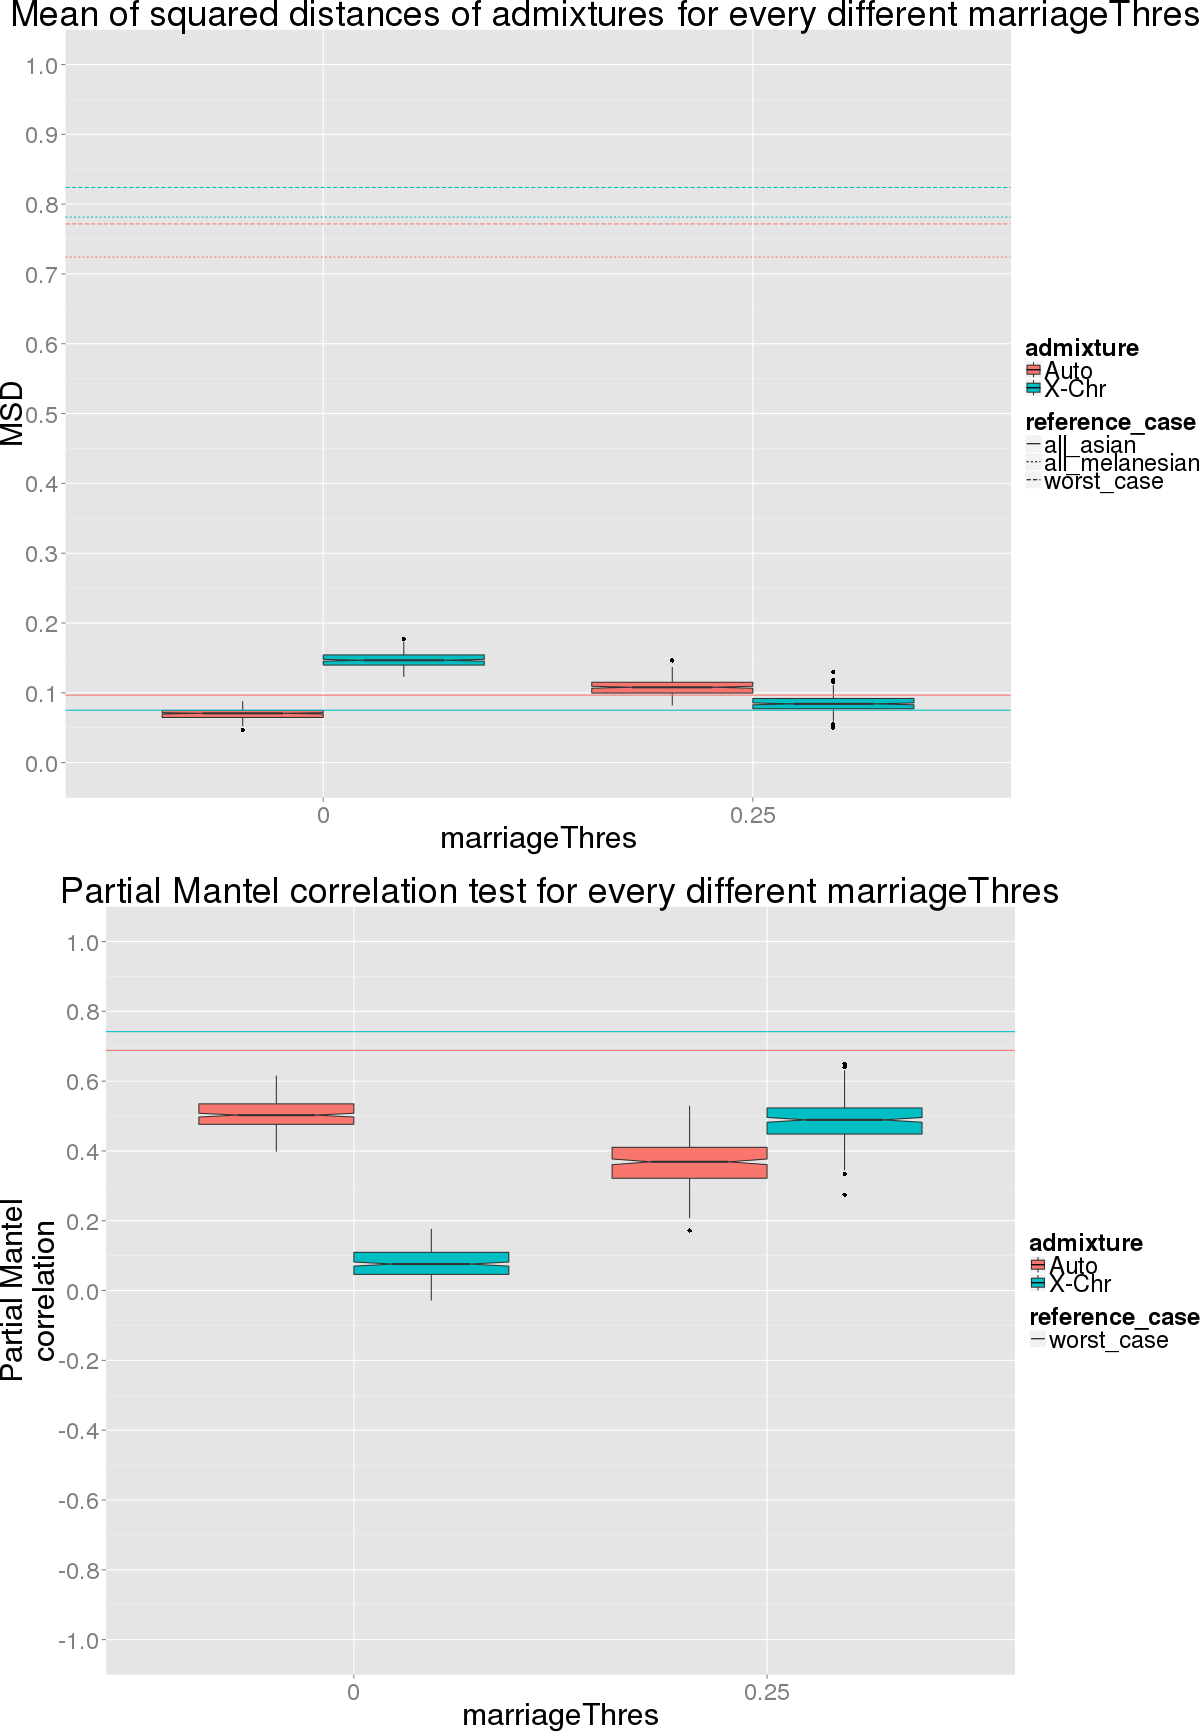
\includegraphics[scale=0.31]{../data/sensit-comp-1d.png}
	\caption{Box-plots of comparisons of simulations vs. real data for a one-dimensional sweep of marriageThres values. Additional lines corresponding to pre-defined extreme reference cases}
	\label{app:sensit-comp-1d}
\end{figure}

\begin{figure}[ht]
	\centering
	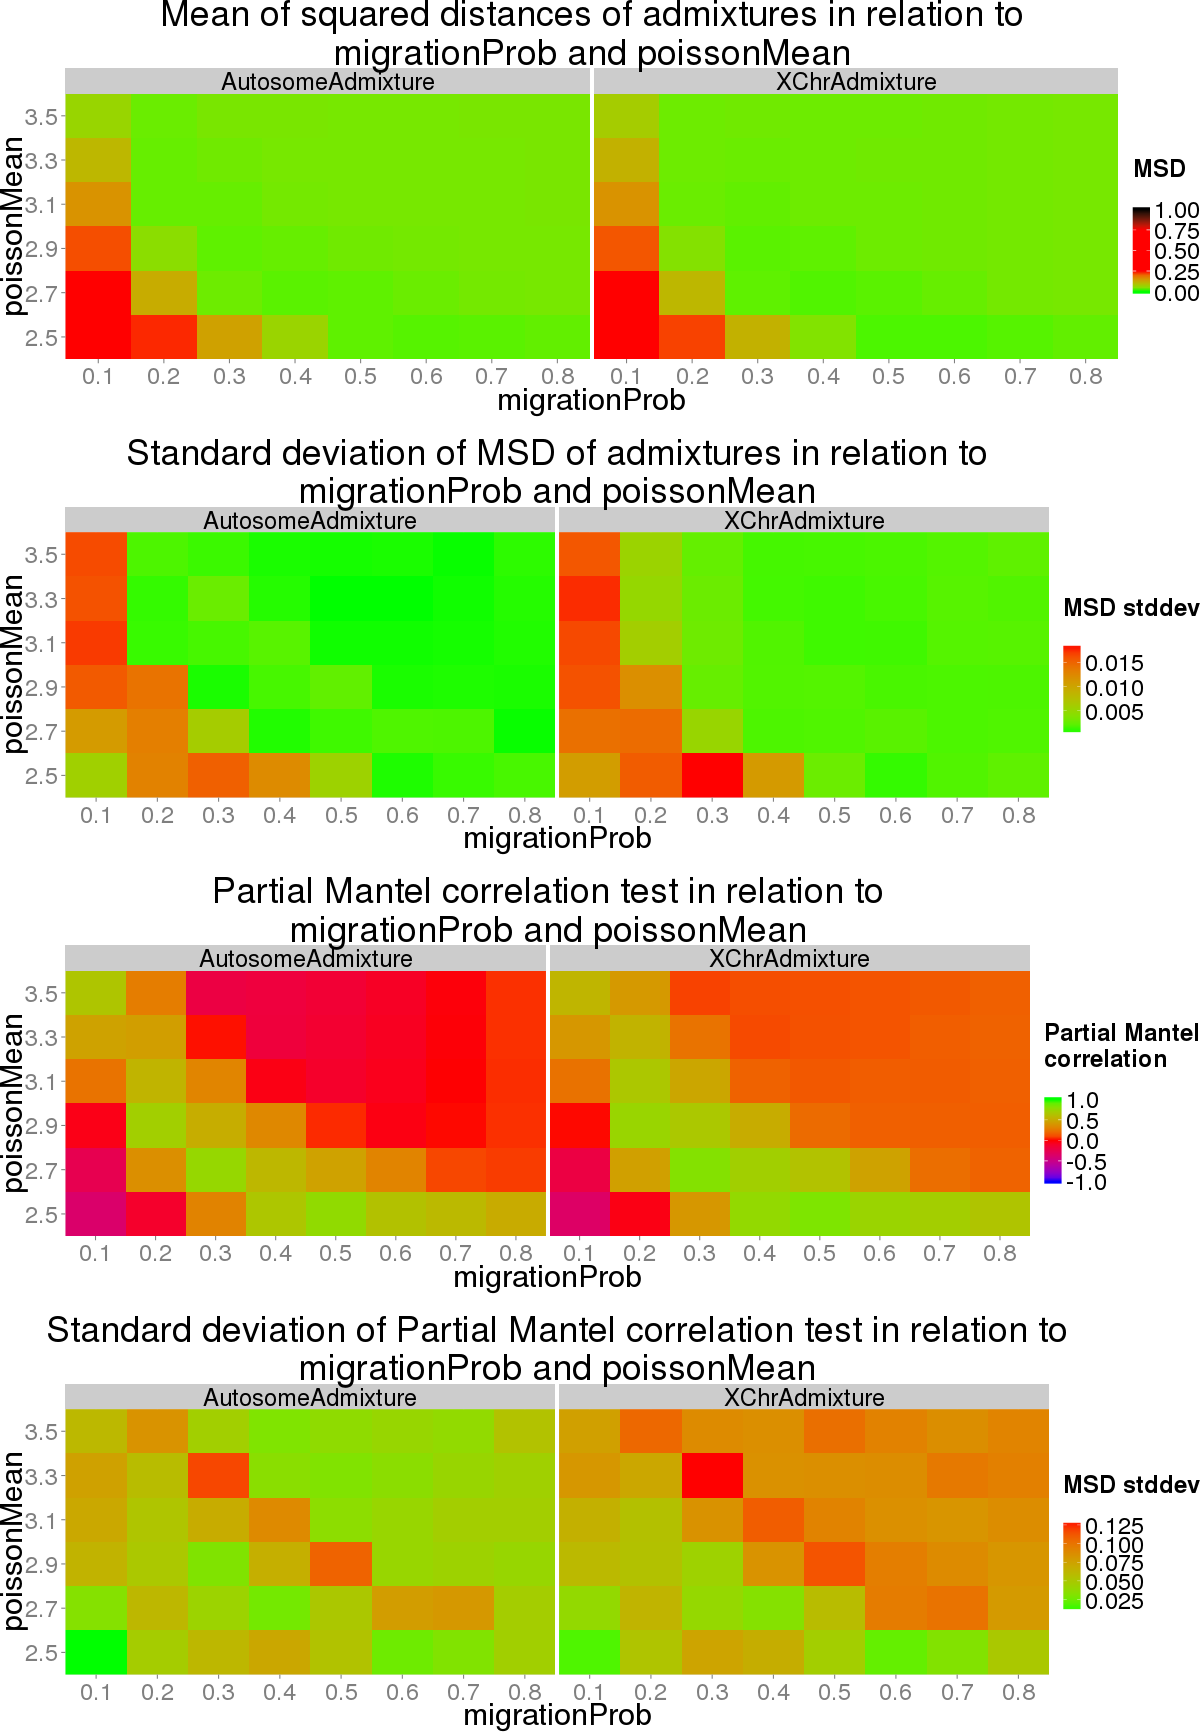
\includegraphics[scale=0.31]{../data/sensit-comp-2d.png}
	\caption{Heat-maps of comparisons and corresponding standard deviations of simulations vs. real data for a two-dimensional sweep of migrationProb and poissonMean values}
	\label{app:sensit-comp-2d}
\end{figure}


\chapter{Benchmarks}
\label{app:bench}

\section{Merging}
\begin{figure}[ht]
	\centering
	%\includegraphics[scale=0.39]{../data/merging-timeByNSimulations.png}
	\caption{Time used by the scripts in relation to the number of simulations merged. Corresponding, in the work-flow, to \texttt{merge.R}}
	\label{app:bench-merging-time}
\end{figure}

\begin{figure}[ht]
	\centering
	%\includegraphics[scale=0.39]{../data/merging-maxMemByNSimulations.png}
	\caption{Maximum memory used by the scripts in relation to the number of simulations analysed. Corresponding, in the work-flow, to \texttt{merge.R}}
	\label{app:bench-merging-mem}
\end{figure}


\section{Analysis}
\begin{figure}[ht]
	\centering
	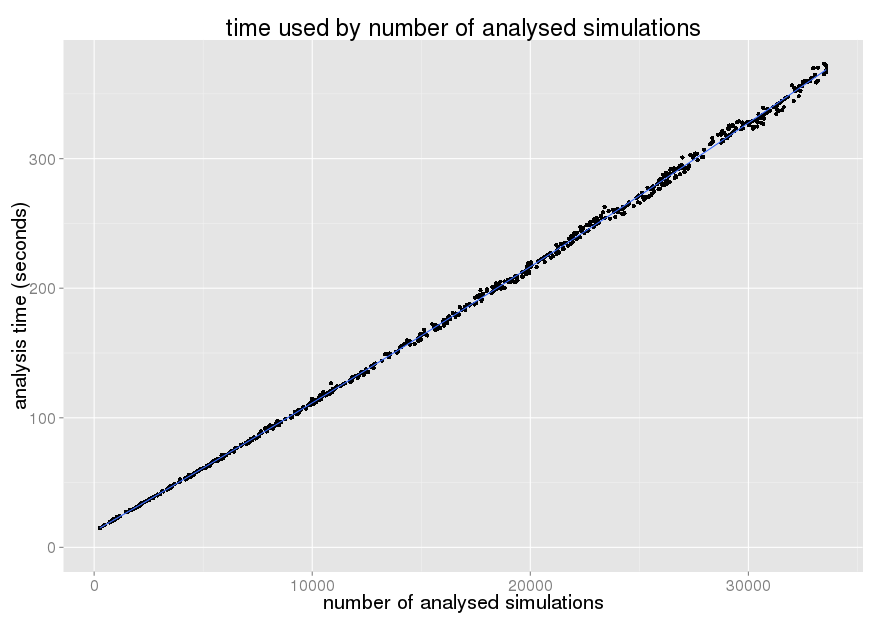
\includegraphics[scale=0.39]{../data/analysis-timeByNSimulations.png}
	\caption{Time used by the scripts in relation to the number of simulations analysed. Corresponding, in the work-flow, to \texttt{analysis.R}, \texttt{sensitivity.R} and the creation of the corresponding output files}
	\label{app:bench-analysis-time}
\end{figure}

\begin{figure}[ht]
	\centering
	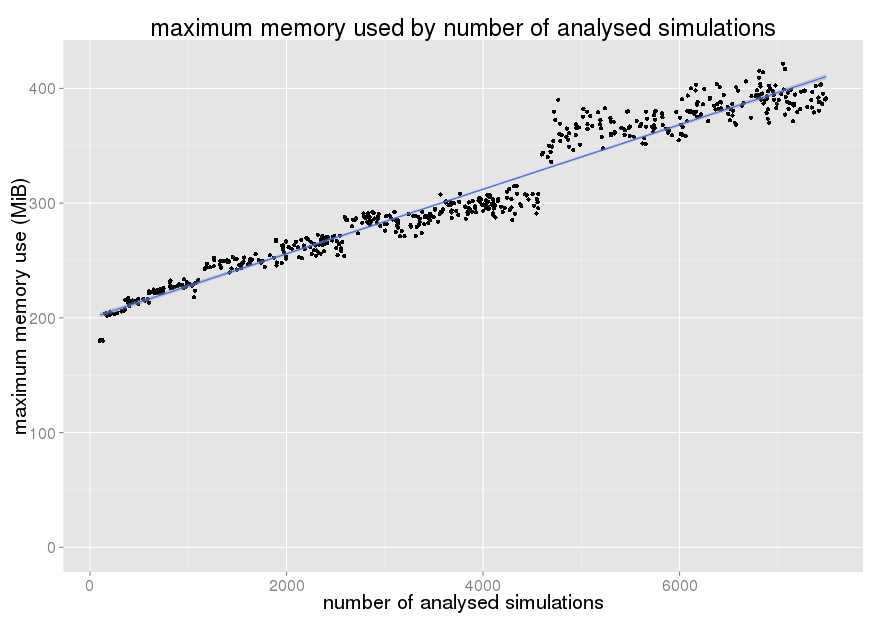
\includegraphics[scale=0.39]{../data/analysis-maxMemByNSimulations.png}
	\caption{Maximum memory used by the scripts in relation to the number of simulations analysed. Corresponding, in the work-flow, to \texttt{analysis.R}, \texttt{sensitivity.R} and the creation of the corresponding output files}
	\label{app:bench-analysis-mem}
\end{figure}

% overview

\end{document}


